% !TEX root = ../main.tex
\providecommand{\text}[1]{\relax\ifmmode\mbox{#1}\else#1\fi}
\chapter{Kiểm thử và đánh giá}
\label{chap:testing-evaluation}

Chương này trình bày cách kiểm thử và đánh giá RabbitCV dựa trên các mục tiêu đã xác định ở Chương 1. Việc đánh giá kết hợp kiểm tra mã nguồn, kiểm thử logic tự động, kiểm thử giao diện bằng trình duyệt và kiểm thử thủ công. Mỗi kết quả được trình bày kèm phạm vi của bằng chứng để tránh suy rộng từ một bài kiểm thử đơn lẻ thành kết luận cho toàn bộ hệ thống.

\section{Công cụ kiểm thử}
\label{sec:testing-tools}

Các công cụ được lựa chọn phù hợp với hệ sinh thái JavaScript của dự án. Mỗi công cụ đảm nhận một phạm vi riêng: Node Test Runner kiểm tra các quy tắc có thể tách biệt, Playwright kiểm tra hành vi giao diện trên trình duyệt, DevTools hỗ trợ quan sát trực tiếp, còn ESLint và Vite Build kiểm tra mã nguồn và khả năng đóng gói.

\subsection{Node Test Runner}

Node Test Runner là công cụ kiểm thử được tích hợp trong Node.js thông qua mô-đun \texttt{node:test}, kết hợp với \texttt{node:assert/strict} để so sánh kết quả thực tế và kết quả mong đợi. Công cụ hỗ trợ ES Modules nên có thể dùng trực tiếp với cấu trúc mã nguồn của RabbitCV mà không cần thêm một khung kiểm thử khác.

Trong dự án, Node Test Runner thực thi 13 tệp với 43 ca kiểm thử. Các ca này gồm hai nhóm chính: kiểm thử hàm độc lập, chẳng hạn chuẩn hóa ngày tháng và kiểm tra PDF; và kiểm tra ở mức mã nguồn, chẳng hạn xác nhận route có middleware, giao diện dùng hook in chung hoặc đặc tả OpenAPI có khai báo xác thực. Vì chuỗi kiểm thử không khởi động MongoDB thật, kết quả không được xem là kiểm thử tích hợp cơ sở dữ liệu toàn hệ thống.

\subsection{Playwright}

Playwright là công cụ tự động hóa trình duyệt, cho phép mô phỏng thao tác mở trang, nhập biểu mẫu, nhấn nút và kiểm tra nội dung hiển thị. RabbitCV sử dụng Playwright Test để chạy 5 bộ tệp kiểm thử (với 26 ca kiểm thử) trên Chromium, tập trung vào kiểm chứng trạng thái hồ sơ ứng tuyển, cơ chế xác thực và điều hướng theo vai trò, tương tác tìm kiếm và biểu mẫu, các thao tác biên tập và bố cục đa mẫu CV, cùng tính năng quản lý tin tuyển dụng và nhận thông báo thời gian thực qua WebSocket.

Các kịch bản sử dụng cơ chế định tuyến \texttt{page.route()} linh hoạt để mô phỏng phản hồi API và các sự kiện mạng. Cách làm này giúp kiểm thử giao diện đạt độ ổn định cao, thời gian thực thi nhanh và không bị phụ thuộc vào dữ liệu tồn tại sẵn trong cơ sở dữ liệu MongoDB, bảo đảm tính độc lập và khả năng lặp lại tuyệt đối của từng kịch bản kiểm thử.


\section{Tổ chức kiểm thử hệ thống}

\subsection{Mục tiêu kiểm thử}

Quá trình kiểm thử RabbitCV hướng đến các mục tiêu sau:

\begin{itemize}
    \item \textbf{Kiểm tra chức năng cốt lõi:} xác minh các quy tắc liên quan đến CV, tìm việc, ứng tuyển, phân quyền, nhắn tin và mô-đun AI.
    \item \textbf{Bảo toàn dữ liệu:} kiểm tra trạng thái công việc, lịch sử ứng tuyển, trạng thái đọc và dữ liệu ẩn theo từng người dùng.
    \item \textbf{Kiểm soát dữ liệu đầu vào:} từ chối PDF sai định dạng hoặc vượt quá 5~MB và làm sạch nội dung có khả năng thực thi.
    \item \textbf{Kiểm tra hiển thị tài liệu:} xác nhận CV tạo trên hệ thống sử dụng kích thước A4 và có quy tắc phục vụ in ấn.
    \item \textbf{Kiểm soát mô-đun AI:} kiểm tra cấu trúc yêu cầu, dữ liệu gửi đi, giới hạn kết quả và cơ chế chỉ áp dụng nội dung sau khi người dùng xác nhận.
    \item \textbf{Đánh giá khả năng đóng gói:} bảo đảm mã nguồn vượt qua kiểm tra tĩnh và có thể tạo bản build frontend.
\end{itemize}

% \subsection{Phạm vi kiểm thử}

% Bảng~\ref{tab:test-scope} phân biệt phạm vi đã được kiểm tra với những nội dung chưa có đủ bằng chứng tự động.

% \begin{table}[H]
%     \centering
%     \small
%     \begin{tabularx}{\textwidth}{|p{0.23\textwidth}|Y|Y|} \hline
%         \textbf{Nhóm} & \textbf{Trong phạm vi hiện tại} & \textbf{Ngoài phạm vi hoặc chưa đầy đủ} \\ \hline
%         Mã nguồn và đóng gói & ESLint, phân giải mô-đun, Vite build và kích thước tài nguyên đầu ra. & Độ bao phủ mã, CI theo commit và kiểm thử trên nhiều hệ điều hành. \\ \hline
%         Logic ứng dụng & Hàm chuẩn hóa, PDF, trạng thái Job, sanitizer, hợp nhất dữ liệu AI và một số hợp đồng cấu hình. & Giao dịch với MongoDB thật và lỗi phát sinh khi nhiều yêu cầu chạy đồng thời. \\ \hline
%         Giao diện trình duyệt & Sáu kịch bản Chromium với API mô phỏng. & Luồng trình duyệt kết nối backend và MongoDB thật; Firefox và WebKit. \\ \hline
%         Hiển thị CV & Quy tắc A4, hook in và cách kết xuất PDF bằng PDF.js. & Ma trận thiết bị, máy in và đo sai số vật lý trên nhiều trình duyệt. \\ \hline
%         AI & Làm sạch dữ liệu, schema đầu ra, hợp nhất dữ liệu và giới hạn phản hồi. & Độ chính xác ngữ nghĩa, tính công bằng và so sánh chất lượng trên bộ dữ liệu độc lập. \\ \hline
%         An toàn và hiệu năng & Một số ràng buộc đầu vào, xác thực route và giới hạn sử dụng. & Kiểm thử xâm nhập, kiểm thử tải, CSRF chuyên sâu và độ bền của Socket.IO trên hạ tầng triển khai. \\ \hline
%     \end{tabularx}
%     \caption{Phạm vi kiểm thử và đánh giá}
%     \label{tab:test-scope}
% \end{table}

\section{Kết quả kiểm thử hệ thống}
\label{sec:system-testing-results}

\subsection{Kiểm thử đơn vị (Node Test Runner)}
\label{subsec:node-test-runner-results}

Bộ kiểm thử logic của RabbitCV được triển khai 13 tệp với tổng cộng 43 ca kiểm thử độc lập, thực thi thông qua lệnh \textit{npm test}. Kết quả ghi nhận toàn bộ 43/43 ca kiểm thử hoàn tất thành công. Bảng~\ref{tab:node-test-inventory} tổng hợp danh mục 13 tệp kiểm thử cùng kết quả chi tiết.

\begingroup
\small
\setlength{\tabcolsep}{3.5pt}
\setlength{\LTcapwidth}{\linewidth}
\begin{longtable}{|>{\centering\arraybackslash}p{0.06\textwidth}|>{\raggedright\arraybackslash}p{0.22\textwidth}|>{\raggedright\arraybackslash}p{0.31\textwidth}|>{\raggedright\arraybackslash}p{0.24\textwidth}|>{\centering\arraybackslash}p{0.08\textwidth}|}
    \caption{Kết quả kiểm thử đơn vị với Node Test Runner} \label{tab:node-test-inventory} \\ \hline
    \textbf{Id} & \textbf{Tên bài kiểm thử} & \textbf{Dữ liệu kiểm thử} & \textbf{Kết quả yêu cầu} & \textbf{Tình trạng} \\ \hline
    \endfirsthead
    \hline
    \textbf{Id} & \textbf{Tên bài kiểm thử} & \textbf{Dữ liệu kiểm thử} & \textbf{Kết quả yêu cầu} & \textbf{Tình trạng} \\ \hline
    \endhead
    \hline
    \endfoot
    \hline
    \endlastfoot
    \multicolumn{5}{|c|}{\textbf{1. a4Layout.test.js}} \\ \hline
    1.1 & Kiểm tra kích thước khổ in A4 của khung CV & Khung hiển thị CV và trang in ấn & Kích thước đạt chuẩn khổ A4 ($210 \times 297$~mm) & Pass \\ \hline
    1.2 & Kiểm tra chức năng tải PDF qua hook in ấn & Nhấn nút "Tải PDF" tại trang chỉnh sửa và danh sách CV & Kích hoạt hook in ấn xuất tệp PDF thành công & Pass \\ \hline
    1.3 & Kiểm tra kết xuất CV PDF tải lên chuẩn A4 & Tệp CV định dạng PDF & Kết xuất tài liệu bằng Canvas qua thư viện PDF.js chuẩn khổ in A4 & Pass \\ \hline
    \multicolumn{5}{|c|}{\textbf{2. pdfValidation.test.js}} \\ \hline
    2.1 & Tiếp nhận tệp PDF hợp lệ và xác định dung lượng & Tệp PDF hợp lệ dung lượng 128~bytes & Xác thực tệp hợp lệ và trả về đúng dung lượng & Pass \\ \hline
    2.2 & Từ chối tệp không đúng định dạng PDF & Tệp định dạng Word (.docx) hoặc nội dung không phải PDF & Từ chối tệp không hợp lệ & Pass \\ \hline
    2.3 & Từ chối tệp PDF vượt quá dung lượng tối đa & Tệp PDF có dung lượng lớn hơn 5~MB & Từ chối do vượt quá dung lượng cho phép & Pass \\ \hline
    \multicolumn{5}{|c|}{\textbf{3. dateInput.test.js}} \\ \hline
    3.1 & Chuẩn hóa định dạng ngày tháng đầu vào & Chuỗi ngày định dạng "2024-05" hoặc "2024-05-15" & Hiển thị đúng định dạng "05/2024" & Pass \\ \hline
    3.2 & Xử lý khoảng thời gian học vấn và kinh nghiệm & Ngày bắt đầu "2020-09" và ngày kết thúc "2024-06" & Xác thực khoảng thời gian hợp lệ & Pass \\ \hline
    3.3 & Xử lý trạng thái công việc đang diễn ra & Chọn công việc đang làm (để trống ngày kết thúc) & Hiển thị nhãn "Hiện tại" & Pass \\ \hline
    3.4 & Phát hiện và từ chối khoảng thời gian nghịch lý & Ngày bắt đầu "2024-01" và kết thúc "2022-01" & Báo lỗi do ngày bắt đầu lớn hơn ngày kết thúc & Pass \\ \hline
    3.5 & Xử lý an toàn giá trị ngày rỗng hoặc sai cú pháp & Dữ liệu ngày rỗng hoặc sai định dạng & Xử lý an toàn, trả về giá trị mặc định & Pass \\ \hline
    \multicolumn{5}{|c|}{\textbf{4. companyUi.test.js}} \\ \hline
    4.1 & Kiểm tra cấu trúc dữ liệu hiển thị hồ sơ doanh nghiệp & Dữ liệu thông tin hồ sơ doanh nghiệp & Hiển thị đầy đủ thông tin chi tiết của công ty & Pass \\ \hline
    4.2 & Hiển thị danh sách tin tuyển dụng của công ty & Danh sách bài đăng tuyển dụng của công ty & Hiển thị đúng danh sách tin và phân trang chính xác & Pass \\ \hline
    4.3 & Kiểm tra cờ trạng thái xác minh doanh nghiệp & Trạng thái xác minh của công ty (đã duyệt hoặc chưa duyệt) & Hiển thị huy hiệu xác thực và cấp quyền tương ứng & Pass \\ \hline
    \multicolumn{5}{|c|}{\textbf{5. jobAvailability.test.js}} \\ \hline
    5.1 & Xác định tin tuyển dụng đang hoạt động (Active) & Tin tuyển dụng đang hoạt động và còn hạn nộp & Hiển thị công khai và cho phép ứng tuyển & Pass \\ \hline
    5.2 & Xác định tin tuyển dụng đã xóa mềm (Deleted) & Tin tuyển dụng đã bị xóa & Ẩn khỏi danh sách tìm kiếm việc làm & Pass \\ \hline
    5.3 & Xác định tin tuyển dụng đã hết hạn (Expired) & Tin tuyển dụng đã quá hạn nộp hồ sơ & Đóng nhận hồ sơ và khóa nút ứng tuyển & Pass \\ \hline
    \multicolumn{5}{|c|}{\textbf{6. jobDeadlineUi.test.js}} \\ \hline
    6.1 & Tính toán và hiển thị số ngày còn lại đến hạn nộp & Hạn nộp còn cách 7 ngày & Hiển thị nhãn thông báo "Còn 7 ngày" & Pass \\ \hline
    6.2 & Hiển thị cảnh báo tin tuyển dụng sắp hết hạn & Hạn nộp còn dưới 24 giờ & Hiển thị cảnh báo màu đỏ "Sắp hết hạn" & Pass \\ \hline
    6.3 & Khóa nút ứng tuyển khi tin đã hết hạn nộp & Hạn nộp đã hết & Khóa nút "Ứng tuyển ngay" & Pass \\ \hline
    \multicolumn{5}{|c|}{\textbf{7. readStatusPersistence.test.js}} \\ \hline
    7.1 & Bảo toàn trạng thái đã đọc của thông báo & Thông báo đã được người dùng nhấn đọc & Lưu trạng thái đã đọc, không mất khi tải lại trang & Pass \\ \hline
    7.2 & Bảo toàn trạng thái đọc tin nhắn riêng từng tài khoản & Người dùng đọc tin nhắn trong cuộc trò chuyện & Cập nhật trạng thái đọc mà không ảnh hưởng đối phương & Pass \\ \hline
    \multicolumn{5}{|c|}{\textbf{8. richTextSanitizer.test.js}} \\ \hline
    8.1 & Bảo toàn thẻ HTML định dạng văn bản an toàn & Văn bản chứa các thẻ định dạng an toàn (in đậm, đoạn văn) & Giữ nguyên định dạng chữ và loại bỏ thuộc tính lạ & Pass \\ \hline
    8.2 & Loại bỏ triệt để mã độc XSS và thẻ nhúng & Văn bản chứa mã độc JavaScript (thẻ script, iframe) & Loại bỏ hoàn toàn mã độc, chỉ giữ văn bản an toàn & Pass \\ \hline
    8.3 & Xử lý an toàn đầu vào không phải chuỗi & Dữ liệu đầu vào rỗng (null hoặc undefined) & Trả về chuỗi rỗng an toàn, không gây lỗi & Pass \\ \hline
    \multicolumn{5}{|c|}{\textbf{9. aiDataSanitizer.test.js}} \\ \hline
    9.1 & Làm sạch văn bản gửi AI và giới hạn độ dài & Đoạn văn bản dài chứa thẻ HTML gửi đến AI & Lọc sạch thẻ HTML và cắt ngắn đúng độ dài quy định & Pass \\ \hline
    9.2 & Nhận diện mã thực thi trong nội dung CV & Văn bản CV chứa đoạn mã thực thi & Nhận diện chính xác văn bản chứa mã lập trình & Pass \\ \hline
    9.3 & Khử định danh thông tin liên hệ trực tiếp trong CV & Hồ sơ CV chứa email và số điện thoại & Ẩn thông tin liên hệ nhạy cảm trước khi gửi sang AI & Pass \\ \hline
    9.4 & Loại bỏ kỹ năng chứa mã thực thi độc hại & Danh sách kỹ năng chứa mục có mã độc & Loại bỏ kỹ năng độc hại, chỉ giữ kỹ năng hợp lệ & Pass \\ \hline
    9.5 & Chuẩn hóa cấu trúc các trường gửi AI & Dữ liệu các mục kinh nghiệm, học vấn gửi sang AI & Chuẩn hóa cấu trúc dữ liệu theo đúng định dạng yêu cầu & Pass \\ \hline
    \multicolumn{5}{|c|}{\textbf{10. resumeAiFill.test.js}} \\ \hline
    10.1 & Hợp nhất kỹ năng gợi ý từ AI an toàn & Kỹ năng hiện có và gợi ý kỹ năng mới từ AI & Bổ sung kỹ năng mới, tự động bỏ qua kỹ năng bị trùng & Pass \\ \hline
    10.2 & Điền phần mô tả còn trống trong mục đã có & Mục dự án có tiêu đề nhưng chưa có mô tả & Điền nội dung mô tả do AI gợi ý vào đúng mục & Pass \\ \hline
    10.3 & Bổ sung kỹ năng mới không cắt xén kỹ năng cũ & Danh sách 10 kỹ năng hiện có và thêm gợi ý từ AI & Giữ nguyên 10 kỹ năng cũ và thêm kỹ năng mới vào cuối & Pass \\ \hline
    10.4 & Điền dữ liệu mẫu khi nhóm nội dung rỗng & Danh sách dự án đang để trống hoàn toàn & Tự động tạo mới dự án mẫu từ gợi ý của AI & Pass \\ \hline
    \multicolumn{5}{|c|}{\textbf{11. aiIntegration.test.js}} \\ \hline
    11.1 & Xác thực cấu hình route AI và Structured Outputs & Yêu cầu gọi dịch vụ AI (Groq API) & Xác thực quyền và trả về dữ liệu đúng chuẩn định dạng & Pass \\ \hline
    11.2 & Kiểm tra giao diện hỗ trợ đúng các luồng AI thực tế & Thao tác gọi tính năng đánh giá và điền CV bằng AI & Gửi yêu cầu đến đúng các luồng xử lý AI tương ứng & Pass \\ \hline
    11.3 & Kiểm tra liên kết trang phỏng vấn AI trên thanh điều hướng & Nhấn vào mục luyện tập phỏng vấn trên menu & Chuyển hướng thành công đến trang phỏng vấn AI & Pass \\ \hline
    11.4 & Kiểm tra phân quyền truy cập tính năng phỏng vấn AI & Tài khoản Doanh nghiệp hoặc Quản trị viên vào trang phỏng vấn & Chặn truy cập và chuyển hướng về đúng trang của vai trò & Pass \\ \hline
    \multicolumn{5}{|c|}{\textbf{12. interviewDataSanitizer.test.js}} \\ \hline
    12.1 & Làm sạch câu trả lời phỏng vấn của ứng viên & Câu trả lời phỏng vấn chứa thẻ HTML hoặc quá dài & Lọc sạch thẻ HTML và giới hạn tối đa 1.200 ký tự & Pass \\ \hline
    12.2 & Chuẩn hóa thang điểm đánh giá phỏng vấn & Điểm số do AI chấm sau câu trả lời & Chuẩn hóa thành số nguyên trong thang điểm từ 0 đến 100 & Pass \\ \hline
    12.3 & Cắt gọn cửa sổ ngữ cảnh lịch sử phỏng vấn & Lịch sử cuộc trò chuyện phỏng vấn dài hơn 30 tin nhắn & Rút gọn, chỉ giữ lại 26 tin nhắn gần nhất trong ngữ cảnh & Pass \\ \hline
    \multicolumn{5}{|c|}{\textbf{13. openapi.test.js}} \\ \hline
    13.1 & Đối chiếu số lượng route thực tế với OpenAPI 3.0 & Toàn bộ danh sách các API đang chạy trên máy chủ & Khớp 100\% với tài liệu đặc tả OpenAPI & Pass \\ \hline
    13.2 & Xác thực cấu hình cookie JWT cho route bảo mật & Các API yêu cầu người dùng đăng nhập & Xác thực thông qua cookie JWT đúng theo đặc tả bảo mật & Pass \\ \hline
\end{longtable}
\endgroup

Dựa trên mục tiêu kiểm chứng, 13 tệp kiểm thử (với 43 ca kiểm thử) được phân thành bốn nhóm trọng tâm chính:
\begin{enumerate}
    \item \textbf{Nhóm kiểm soát an toàn và tính năng AI (5 tệp):}
    Bao gồm các bài kiểm thử trong \textit{aiDataSanitizer.test.js}, \textit{richTextSanitizer.test.js}, \textit{resumeAiFill.test.js}, \textit{aiIntegration.test.js} và \textit{interviewDataSanitizer.test.js}. Bộ lọc \textit{aiDataSanitizer} giúp loại bỏ thông tin liên hệ nhạy cảm (email, số điện thoại, địa chỉ) trước khi gửi sang mô hình AI nhằm bảo vệ quyền riêng tư của ứng viên; bộ lọc \textit{richTextSanitizer} loại bỏ triệt để mã độc XSS trong nội dung văn bản; \textit{resumeAiFill} kiểm tra cơ chế bổ sung kỹ năng gợi ý vào CV một cách an toàn mà không ghi đè dữ liệu người dùng đã có; đồng thời kiểm tra luồng kết nối, làm sạch phản hồi và chuẩn hóa thang điểm đánh giá trong chức năng luyện tập phỏng vấn AI.
    
    \item \textbf{Nhóm kiểm thử hiển thị và xử lý tệp tin (3 tệp):}
    Bao gồm các tệp \textit{a4Layout.test.js}, \textit{pdfValidation.test.js} và \textit{dateInput.test.js}. Các bài kiểm thử xác minh tệp PDF tải lên tuân thủ đúng định dạng A4 và dung lượng không vượt quá 5~MB; xác nhận khung bao đáp ứng chuẩn kích thước khổ in A4 ($210 \times 297$~mm), áp dụng quy tắc ngắt trang và kết xuất PDF tải lên trực tiếp trên canvas bằng PDF.js; đồng thời chuẩn hóa định dạng ngày tháng đầu vào cho các mốc thời gian học vấn, kinh nghiệm và xử lý trạng thái công việc hiện tại.

    \item \textbf{Nhóm quy tắc nghiệp vụ và giao diện người dùng (4 tệp):}
    Tập hợp 4 tệp kiểm thử gồm \textit{jobAvailability.test.js}, \textit{jobDeadlineUi.test.js}, \textit{companyUi.test.js} và \textit{readStatusPersistence.test.js}. Các bài kiểm thử kiểm tra thuật toán phân loại và hiển thị trạng thái tin tuyển dụng (tin đã xóa, tin đang hoạt động hoặc đã hết hạn), hiển thị số ngày còn lại và tự động khóa tính năng nộp đơn khi tin hết hạn; đồng thời đảm bảo trạng thái đã đọc của tin nhắn và thông báo được lưu trữ bền vững, không bị mất khi người dùng tải lại trang.

    \item \textbf{Nhóm đặc tả và cấu hình API hệ thống (1 tệp):}
    Bao gồm tệp \textit{openapi.test.js} (2 ca kiểm thử). Bài kiểm thử thực hiện đối chiếu toàn bộ các route HTTP thực tế của hệ thống với tài liệu đặc tả OpenAPI 3.0, đồng thời xác thực cơ chế bảo mật của các endpoint yêu cầu xác thực người dùng thông qua cookie JWT.
\end{enumerate}

\begin{figure}[H]
    \centering
    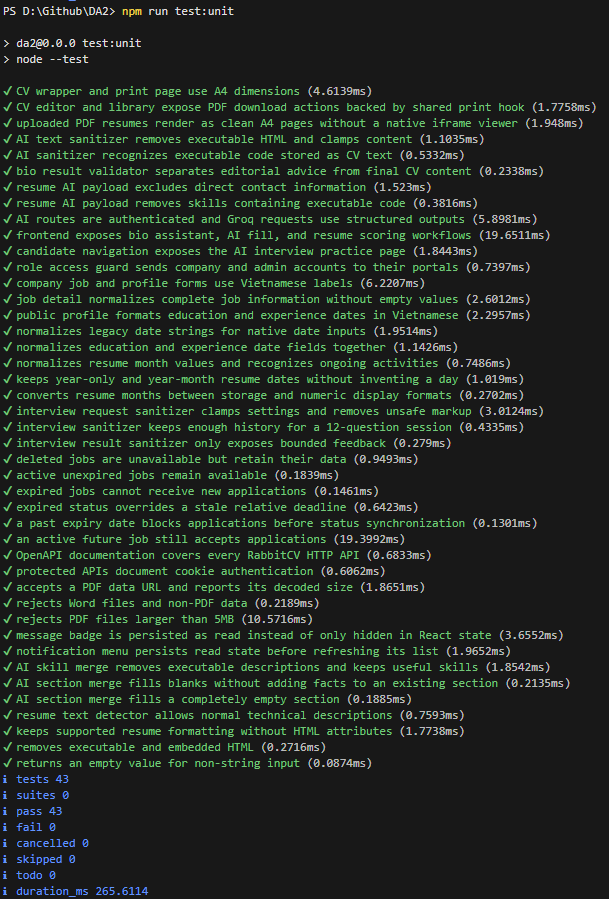
\includegraphics[
        width=1\linewidth,
        height=0.7\textheight,
        keepaspectratio
    ]{img/NodeTestResult.png}
    \caption{Kết quả Node Test Runner}
    \label{fig:nodetestrunnerresult}
\end{figure}

Kết quả thực thi minh họa tại Hình~\ref{fig:nodetestrunnerresult} cho thấy bộ kiểm thử tự động Node Test Runner đã chạy đạt 43/43 ca kiểm thử thành công, không ghi nhận bất kỳ trường hợp lỗi hay bị bỏ qua. Với tổng thời gian thực thi chỉ khoảng 266~ms trên toàn bộ 13 tệp kiểm thử, việc khai thác trình chạy kiểm thử tích hợp sẵn trong Node.js đã tối ưu hóa vượt bậc tốc độ phản hồi so với các khung kiểm thử truyền thống, tạo điều kiện thuận lợi cho chu trình phản hồi nhanh trong quá trình phát triển mã nguồn.

Nhìn chung, các ca kiểm thử của Node Test Runner vận hành trong môi trường bộ nhớ cô lập với dữ liệu giả lập, đóng vai trò như một chốt chặn kiểm soát vững chắc cho toàn bộ các hàm thuật toán độc lập và cấu trúc dữ liệu nền tảng trước khi hệ thống được đưa vào kiểm thử tương tác trên trình duyệt thực tế.

\subsection{Playwright}
\label{subsec:playwright-results}

Để kiểm chứng hành vi của ứng dụng trên môi trường trình duyệt thực tế, hệ thống sử dụng khung kiểm thử tự động hóa \textbf{Playwright Test} điều khiển trình duyệt Chromium. Bộ kiểm thử tập trung vào thẩm định toàn diện các luồng tương tác người dùng, cơ chế xác thực và điều hướng theo vai trò, quy trình duyệt hồ sơ ứng tuyển, các thao tác biên tập và kéo thả bố cục CV trên nhiều mẫu giao diện, cùng cơ chế đồng bộ dữ liệu việc làm và nhận thông báo thời gian thực qua WebSocket.

Bảng~\ref{tab:playwright-results} trình bày chi tiết 26 ca kiểm thử thuộc 5 tệp kiểm thử tự động trên trình duyệt Chromium. Toàn bộ các ca kiểm thử được lựa chọn đều đạt kết quả Pass trong lần chạy được ghi nhận, đồng thời kết quả thực thi thực tế cũng được thể hiện đồng bộ trong báo cáo Playwright ở mục tiếp theo.

\begingroup
\small
\setlength{\tabcolsep}{3.5pt}
\setlength{\LTcapwidth}{\linewidth}
\begin{longtable}{|>{\centering\arraybackslash}p{0.05\textwidth}|>{\raggedright\arraybackslash}p{0.20\textwidth}|>{\raggedright\arraybackslash}p{0.35\textwidth}|>{\raggedright\arraybackslash}p{0.24\textwidth}|>{\centering\arraybackslash}p{0.07\textwidth}|}
    \caption{Kết quả kiểm thử giao diện và phân quyền bằng \mbox{Playwright}} \label{tab:playwright-results} \\ \hline
    \textbf{Id} & \textbf{Tên bài kiểm thử} & \textbf{Các bước thực hiện} & \textbf{Kết quả mong đợi} & \textbf{Tình trạng} \\ \hline
    \endfirsthead
    \hline
    \textbf{Id} & \textbf{Tên bài kiểm thử} & \textbf{Các bước thực hiện} & \textbf{Kết quả mong đợi} & \textbf{Tình trạng} \\ \hline
    \endhead
    \hline
    \endfoot
    \hline
    \endlastfoot
    \multicolumn{5}{|c|}{\textbf{1. application-status.spec.js}} \\ \hline
    1.1 & Xác nhận từ chối và khóa trạng thái hồ sơ & 1. Mở danh sách hồ sơ ứng viên. \newline 2. Bấm nút "Từ chối" trên hồ sơ. \newline 3. Bấm xác nhận trên hộp thoại. & Hồ sơ chuyển sang trạng thái "Đã từ chối" và các nút thao tác bị vô hiệu hóa & Pass \\ \hline
    1.2 & Giữ nguyên trạng thái khi từ chối thất bại & 1. Mở hồ sơ ứng viên và chọn "Từ chối". \newline 2. Giả lập máy chủ phản hồi lỗi cập nhật (500). \newline 3. Bấm xác nhận từ chối hồ sơ. & Hiển thị thông báo lỗi và giữ nguyên trạng thái "Chờ duyệt" ban đầu & Pass \\ \hline
    \multicolumn{5}{|c|}{\textbf{2. auth-routing.spec.js}} \\ \hline
    2.1 & Hiển thị trang chủ chào mừng & 1. Khởi tạo phiên duyệt web chưa đăng nhập. \newline 2. Truy cập vào đường dẫn trang chủ (/). & Hiển thị đầy đủ thông tin giới thiệu và các nút điều hướng Đăng nhập / Đăng ký & Pass \\ \hline
    2.2 & Kiểm tra form đăng nhập trống & 1. Mở biểu mẫu đăng nhập (/login). \newline 2. Để trống tài khoản và mật khẩu. \newline 3. Bấm nút "Đăng nhập". & Ngăn gửi biểu mẫu và hiển thị thông báo yêu cầu nhập đầy đủ thông tin & Pass \\ \hline
    2.3 & Đăng nhập vai trò Ứng viên & 1. Mở trang đăng nhập (/login). \newline 2. Nhập tài khoản Ứng viên hợp lệ. \newline 3. Bấm nút "Đăng nhập". & Đăng nhập thành công và tự động chuyển hướng người dùng vào trang /MainMenu & Pass \\ \hline
    2.4 & Đăng nhập vai trò Doanh nghiệp & 1. Mở trang đăng nhập (/login). \newline 2. Nhập tài khoản Doanh nghiệp hợp lệ. \newline 3. Bấm nút "Đăng nhập". & Đăng nhập thành công và chuyển hướng đến trang /CompanyDashboard & Pass \\ \hline
    2.5 & Đăng nhập vai trò Quản trị viên & 1. Mở trang đăng nhập (/login). \newline 2. Nhập tài khoản Quản trị viên hợp lệ. \newline 3. Bấm nút "Đăng nhập". & Đăng nhập thành công và chuyển hướng vào bảng điều khiển /admin & Pass \\ \hline
    2.6 & Chặn ứng viên vào trang quản trị & 1. Đăng nhập bằng tài khoản Ứng viên. \newline 2. Nhập trực tiếp URL /admin trên trình duyệt. \newline 3. Nhấn phím Enter để truy cập. & RoleAccessGuard chặn truy cập và tự động điều hướng người dùng về /MainMenu & Pass \\ \hline
    \multicolumn{5}{|c|}{\textbf{3. cv-editing.spec.js}} \\ \hline
    3.1 & Sửa mục tùy chỉnh và hoàn tác/làm lại & 1. Đổi tên mục tùy chỉnh trong CV. \newline 2. Bấm nút "Hoàn tác" (Undo). \newline 3. Bấm nút "Làm lại" (Redo). & Tên mục khôi phục về tên cũ khi hoàn tác và đổi sang tên mới khi làm lại & Pass \\ \hline
    3.2 & Kéo thả sắp xếp bố cục CV & 1. Nhấp giữ một khối nội dung trên CV. \newline 2. Kéo thả sang vị trí mong muốn ở cột khác. \newline 3. Nhả chuột để hoàn tất sắp xếp. & Thứ tự các khối nội dung được cập nhật chính xác và đồng bộ trên bản xem trước & Pass \\ \hline
    3.3 & Xóa và khôi phục mục tùy chỉnh & 1. Bấm nút xóa một mục tùy chỉnh trong CV. \newline 2. Bấm nút "Hoàn tác" (Undo). & Mục tùy chỉnh bị xóa khỏi CV và được khôi phục nguyên vẹn sau khi hoàn tác & Pass \\ \hline
    3.4 & AI điền CV và hoàn tác/làm lại & 1. Bấm kích hoạt tính năng AI tự động điền CV. \newline 2. Chờ áp dụng nội dung AI gợi ý vào CV. \newline 3. Bấm nút "Hoàn tác" (Undo). & Nội dung do AI tạo được điền vào CV và khôi phục lại trạng thái cũ khi hoàn tác & Pass \\ \hline
    3.5 & Lưu CV mới và giữ lịch sử hoàn tác & 1. Mở trình chỉnh sửa CV mới. \newline 2. Thêm nhóm nội dung và một mục trong nhóm. \newline 3. Nhấn lưu với API mô phỏng thành công. \newline 4. Kiểm tra URL chuyển sang CV có mã định danh. \newline 5. Thực hiện hoàn tác và làm lại. & URL chuyển sang CV đã tạo; lịch sử hoàn tác/làm lại vẫn được duy trì sau phản hồi lưu mô phỏng & Pass \\ \hline
    3.6 & Đồng bộ editor tiểu sử khi hoàn tác & 1. Nhập chỉnh sửa văn bản tiểu sử. \newline 2. Bấm nút "Hoàn tác" (Undo). & Nội dung tiểu sử trong trình soạn thảo đồng bộ quay về đúng văn bản ban đầu & Pass \\ \hline
    3.7 & Quản lý nhóm mục tùy chỉnh và chi tiết & 1. Thêm mục chi tiết vào nhóm tùy chỉnh. \newline 2. Bật/tắt công tắc ẩn/hiện các trường. & Bản xem trước CV hiển thị hoặc ẩn chính xác các trường thông tin theo cấu hình & Pass \\ \hline
    3.8 & Thêm và lưu tên kỹ năng & 1. Mở nhóm kỹ năng và thêm tên kỹ năng mới. \newline 2. Thực hiện hoàn tác và làm lại. \newline 3. Nhấn lưu. \newline 4. Kiểm tra dữ liệu gửi đến API mô phỏng. & Dữ liệu gửi đi chứa tên kỹ năng, không chứa trường mô tả hoặc mức độ cũ & Pass \\ \hline
    3.9 & Hiển thị kỹ năng trên template classic & 1. Mở bản CV có chứa nhóm kỹ năng. \newline 2. Bấm chuyển sang mẫu CV Classic (Cổ điển). & Khối kỹ năng hiển thị đúng định dạng và phong cách trình bày của mẫu Classic & Pass \\ \hline
    3.10 & Hiển thị kỹ năng trên các template còn lại (Modern, Professional, Elegant, Creative, Compact) (5 test) & 1. Mở bản CV có chứa nhóm kỹ năng. \newline 2. Lần lượt bấm chuyển sang các mẫu CV: Modern, Professional, Elegant, Creative và Compact. & Khối kỹ năng hiển thị đồng bộ, đúng định dạng và bố cục đặc trưng của từng mẫu template & Pass \\ \hline
    \multicolumn{5}{|c|}{\textbf{4. job-visibility.spec.js}} \\ \hline
    4.1 & Đồng bộ ẩn/hiện/xóa tin tuyển dụng & 1. Mở giao diện quản trị và danh sách việc làm của ứng viên. \newline 2. Ẩn tin và kích hoạt cập nhật danh sách ứng viên. \newline 3. Bỏ ẩn tin và cập nhật lại danh sách. \newline 4. Xóa mềm tin và cập nhật danh sách. & Tin biến mất khi bị ẩn hoặc xóa mềm và xuất hiện lại khi bỏ ẩn trong dữ liệu mô phỏng & Pass \\ \hline
    4.2 & Tự động cập nhật danh sách việc làm qua polling & 1. Mở danh sách việc làm của ứng viên. \newline 2. Chuyển tin sang trạng thái xóa mềm trong dữ liệu API mô phỏng. \newline 3. Tua đồng hồ kiểm thử đến chu kỳ polling tiếp theo. & Danh sách được làm mới và loại bỏ tin đã xóa mềm mà không cần tải lại trang & Pass \\ \hline
    4.3 & Báo lỗi khi tin tuyển dụng bị gỡ & 1. Sao chép liên kết của một tin đã bị xóa. \newline 2. Truy cập trực tiếp URL đó trên trình duyệt. & Hệ thống báo lỗi và hiển thị thông báo "Không tìm thấy tin tuyển dụng" & Pass \\ \hline
    \multicolumn{5}{|c|}{\textbf{5. notifications-realtime.spec.js}} \\ \hline
    5.1 & Nhận thông báo, chống trùng và kết nối lại & 1. Mở trang thông báo với API và WebSocket mô phỏng. \newline 2. Gửi sự kiện thông báo mới. \newline 3. Gửi lại cùng sự kiện. \newline 4. Ngắt kết nối và bổ sung thông báo trong API mô phỏng. \newline 5. Chờ kết nối lại và kiểm tra số chưa đọc. \newline 6. Nhấn chuông thông báo. & Danh sách, huy hiệu và toast được cập nhật; sự kiện trùng không tăng số lượng; kết nối lại đồng bộ số chưa đọc từ API; nhấn chuông xóa huy hiệu & Pass \\ \hline
\end{longtable}
\endgroup

Các cơ chế trọng yếu được kiểm chứng qua bộ kiểm thử Playwright bao gồm:
\begin{itemize}
    \item \textbf{Kiểm soát quy trình tuyển dụng và trạng thái hồ sơ:} Đảm bảo tính nhất quán của trạng thái ứng tuyển. Khi doanh nghiệp từ chối hồ sơ, hệ thống bắt buộc hiển thị hộp thoại xác nhận và khóa trạng thái vĩnh viễn để tránh sai sót; trường hợp máy chủ gặp sự cố, giao diện tự động duy trì trạng thái an toàn.
    \item \textbf{Phân luồng đa vai trò và rào chắn phân quyền (RoleAccessGuard):} Bộ định tuyến phản hồi chính xác với thông tin vai trò từ API xác thực, tự động điều hướng người dùng về đúng trang nghiệp vụ. Cơ chế bảo vệ cổng quản trị ngăn chặn triệt để hành vi truy cập trái phép của ứng viên vào đường dẫn \texttt{/admin}.
    \item \textbf{Khả năng tương tác và chỉnh sửa CV nâng cao:} Kiểm chứng cơ chế kéo-thả (\textit{Drag-and-Drop}) linh hoạt giữa các cột, tính năng hoàn tác/làm lại (\textit{Undo/Redo}) đa cấp cho cả thao tác thủ công lẫn nội dung điền tự động từ AI, đồng thời kiểm tra sự hiển thị đồng bộ của các khối kỹ năng trên cả 6 mẫu template CV khác nhau.
    \item \textbf{Đồng bộ trạng thái việc làm và thông báo thời gian thực:} Cơ chế polling định kỳ bảo đảm danh sách việc làm luôn hiển thị chính xác các tin còn hiệu lực; đồng thời kết nối WebSocket qua Socket.IO truyền phát thông báo ngay lập tức đến ứng viên mà không làm trùng lặp thông báo trên giao diện.
\end{itemize}

\subsection{Kết quả thực thi Playwright}
\label{subsec:playwright-execution-details}

Toàn bộ 5 tệp kịch bản kiểm thử (gồm 26 ca kiểm thử) được thực thi tự động trên môi trường trình duyệt Chromium với cơ chế cô lập phiên làm việc hoàn toàn. Giao diện báo cáo HTML của Playwright (\textit{Playwright HTML Reporter}) ghi nhận kết quả thực thi chi tiết được minh họa tuần tự tại Hình~\ref{fig:playwright-report-1} và Hình~\ref{fig:playwright-report-2}.

\begin{figure}[H]
    \centering
    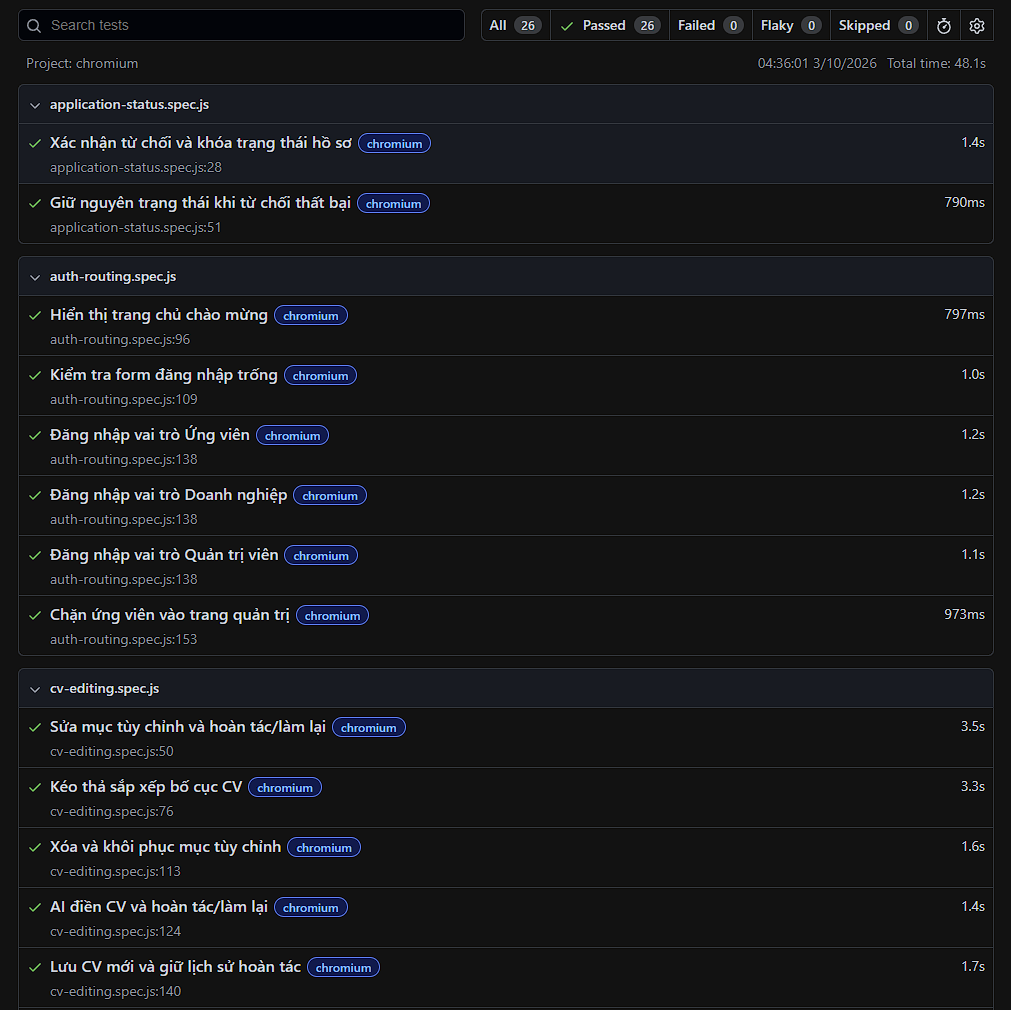
\includegraphics[width=0.92\linewidth,keepaspectratio]{img/Playwright_1.png}
    \caption{Báo cáo thực thi Playwright}
    \label{fig:playwright-report-1}
\end{figure}

\begin{figure}[H]
    \centering
    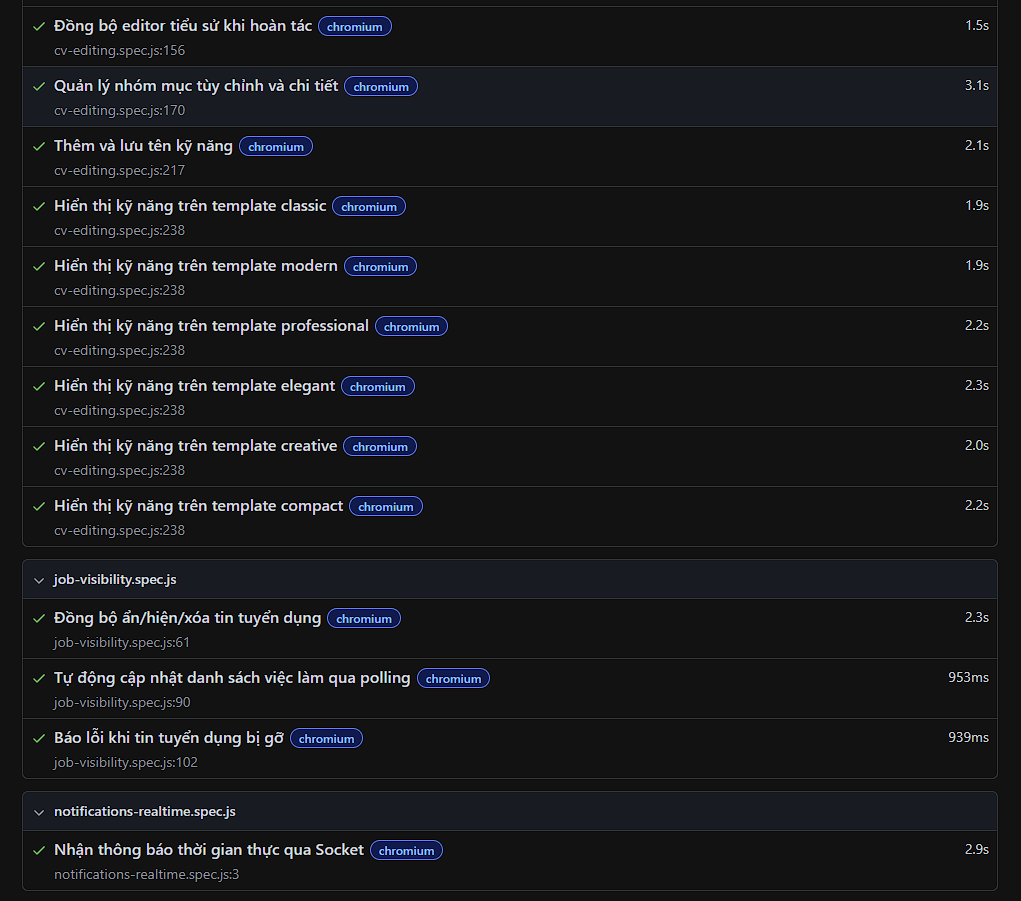
\includegraphics[width=0.92\linewidth,keepaspectratio]{img/Playwright_2.png}
    \caption{Báo cáo thực thi Playwright}
    \label{fig:playwright-report-2}
\end{figure}

Kết quả thực nghiệm từ báo cáo tổng thể cho thấy toàn bộ \textbf{26/26 ca kiểm thử đều hoàn tất thành công} (\textit{Passed 26, Failed 0, Flaky 0, Skipped 0}) với tổng thời gian thực thi là 48.1 giây trên trình duyệt Chromium. Trình kiểm thử tận dụng cơ chế chạy đa tiến trình song song, cho phép đẩy nhanh tiến độ kiểm tra toàn diện ứng dụng web mà vẫn đảm bảo tính chính xác và độ cô lập tuyệt đối giữa các ngữ cảnh trình duyệt. Tỷ lệ hoàn thành đạt 100\% mà không xuất hiện bất kỳ ca kiểm thử chập chờn (\textit{flaky}) nào khẳng định tính ổn định cao của giao diện người dùng và cơ chế đồng bộ dữ liệu.

% \subsection{Đánh giá hiệu năng}

% Bên cạnh tính chính xác của kết quả kiểm thử, hiệu năng và khả năng mở rộng của hệ thống kiểm thử cũng là yếu tố then chốt được xem xét. Bảng~\ref{tab:playwright-stats} tổng hợp các chỉ số về độ tin cậy, tốc độ thực thi và khả năng tài nguyên của bộ kiểm thử Playwright.

% \begin{table}[H]
%     \centering
%     \caption{Thống kê hiệu năng và độ tin cậy của bộ kiểm thử Playwright}
%     \label{tab:playwright-stats}
%     \begin{tabular}{@{}llr@{}}
%         \toprule
%         Chỉ số & Mô tả & Giá trị \\
%         \midrule
%         \multicolumn{2}{l}{\textbf{Kết quả thực thi}} & \\
%         Kịch bản đã chạy & Tổng số ca kiểm thử được thực thi & 27 \\
%         Kịch bản thành công & Số ca kiểm thử hoàn tất thành công & 27 \\
%         Kịch bản lỗi & Số ca kiểm thử thất bại & 0 \\
%         Kịch bản không ổn định & Số ca kiểm thử bị lỗi ngẫu nhiên & 0 \\
%         Kịch bản bị bỏ qua & Số ca kiểm thử không được thực thi & 0 \\
%         \midrule
%         \multicolumn{2}{l}{\textbf{Hiệu năng thực thi}} & \\
%         Tổng thời gian thực thi & Thời gian xử lý toàn bộ 27 kịch bản & 47.4 giây \\
%         Thời gian trung bình / kịch bản & Thời gian trung bình cho mỗi ca kiểm thử & 1.75 giây \\
%         Thời gian phản hồi nhanh nhất & Kịch bản chạy nhanh nhất & 0.71 giây \\
%         Thời gian phản hồi chậm nhất & Kịch bản chạy chậm nhất & 4.20 giây \\
%         \midrule
%         \multicolumn{2}{l}{\textbf{Tài nguyên sử dụng}} & \\
%         Số tiến trình song song & Cấu hình trình kiểm thử & 3 \\
%         Tải CPU & Mức sử dụng bộ xử lý trong quá trình chạy & \(\leq 60\)\%
%         \\
%         Tải bộ nhớ & Mức sử dụng RAM & \(\leq 800\) MB
%         \\
%         \bottomrule
%     \end{tabular}
% \end{table}

% Kết quả đánh giá cho thấy bộ kiểm thử Playwright đạt hiệu năng cao và độ tin cậy tuyệt đối cho các kịch bản kiểm thử End-to-End được xác định (Bảng~\ref{tab:playwright-stats}). Với toàn bộ 27/27 kịch bản đều thành công, không ghi nhận bất kỳ ca kiểm thử lỗi hay lỗi không ổn định nào, bộ kiểm thử khẳng định tính ổn định và đáng tin cậy cho các quy trình nghiệp vụ cốt lõi của hệ thống.

% \clearpage
